\documentclass[border=4pt]{standalone}
\usepackage{amsmath,amssymb,pgfplots}\pgfplotsset{compat=1.18}
\definecolor{figB}{RGB}{31,90,166}\definecolor{figR}{RGB}{176,48,48}\definecolor{figG}{RGB}{46,125,50}\definecolor{figO}{RGB}{214,120,20}
\begin{document}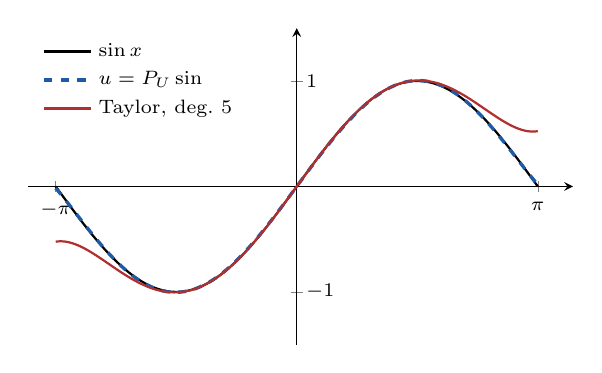
\begin{tikzpicture}
\begin{axis}[width=8.5cm,height=5.6cm,axis lines=middle,axis line style={-stealth,thin},
  xmin=-3.5,xmax=3.6,ymin=-1.5,ymax=1.5,xtick={-3.1416,3.1416},xticklabels={$-\pi$,$\pi$},ytick={-1,1},
  ticklabel style={font=\scriptsize},y tick label style={anchor=west,xshift=2pt},
  legend style={font=\scriptsize,at={(0.01,0.99)},anchor=north west,draw=none,fill=white,fill opacity=0.85,text opacity=1,cells={anchor=west}},
  samples=200,domain=-3.1416:3.1416]
\addplot[black,thick] {sin(deg(x))}; \addlegendentry{$\sin x$}
\addplot[figB,very thick,dashed] {0.987862*x-0.155271*x^3+0.00564312*x^5}; \addlegendentry{$u=P_U\sin$}
\addplot[figR,thick] {x-x^3/6+x^5/120}; \addlegendentry{Taylor, deg.~$5$}
\end{axis}\end{tikzpicture}\end{document}
